%% This file explains the options available to you for editing the file
%% main.tex.

%% The commands in this file allow you to specify options such as
%% spacing, double-sided printing, a draft copy, etc.   By default, 12pt
%% and lgrind are included; lgrind is the 2e style for including code in
%% your thesis.

%% \documentclass[12pt]{mitthesis}
%% \usepackage{lgrind}
%% \pagestyle{plain}

%% You can add options in the documentclass line as follows:

%% 	o  singlespace
%% 	\documentclass[12pt,singlespace]{mitthesis}
	
%% 	o  twoside
%% 	\documentclass[12pt,twoside]{mitthesis}

%% 	o  draft   (make sure to change the pagestyle to drafthead as well)
%% 	\documentclass[12pt,draft]{mitthesis}
%% 	\usepackage{lgrind}
%% 	\pagestyle{drafthead}

%% 	o vi   (for course vi and course viii theses)
%% 	\documentclass[12pt,vi]{mitthesis}

%% Any options you would use for report.sty will work here as well.


%% You should not need to change the first three lines and last two lines
%% below.  Be sure to include an \include command for each file you are
%% including in your thesis.
  
%% % -*-latex-*-
% 
% For questions, comments, concerns or complaints:
% thesis@mit.edu
% 
%
% $Log: cover.tex,v $
% Revision 1.9  2019/08/06 14:18:15  cmalin
% Replaced sample content with non-specific text.
%
% Revision 1.8  2008/05/13 15:02:15  jdreed
% Degree month is June, not May.  Added note about prevdegrees.
% Arthur Smith's title updated
%
% Revision 1.7  2001/02/08 18:53:16  boojum
% changed some \newpages to \cleardoublepages
%
% Revision 1.6  1999/10/21 14:49:31  boojum
% changed comment referring to documentstyle
%
% Revision 1.5  1999/10/21 14:39:04  boojum
% *** empty log message ***
%
% Revision 1.4  1997/04/18  17:54:10  othomas
% added page numbers on abstract and cover, and made 1 abstract
% page the default rather than 2.  (anne hunter tells me this
% is the new institute standard.)
%
% Revision 1.4  1997/04/18  17:54:10  othomas
% added page numbers on abstract and cover, and made 1 abstract
% page the default rather than 2.  (anne hunter tells me this
% is the new institute standard.)
%
% Revision 1.3  93/05/17  17:06:29  starflt
% Added acknowledgements section (suggested by tompalka)
% 
% Revision 1.2  92/04/22  13:13:13  epeisach
% Fixes for 1991 course 6 requirements
% Phrase "and to grant others the right to do so" has been added to 
% permission clause
% Second copy of abstract is not counted as separate pages so numbering works
% out
% 
% Revision 1.1  92/04/22  13:08:20  epeisach

% NOTE:
% These templates make an effort to conform to the MIT Thesis specifications,
% however the specifications can change. We recommend that you verify the
% layout of your title page with your thesis advisor and/or the MIT 
% Libraries before printing your final copy.
\title{MIT Thesis Template in Overleaf}

\author{Tim Beaver}
% If you wish to list your previous degrees on the cover page, use the 
% previous degrees command:
%       \prevdegrees{A.A., Harvard University (1985)}
% You can use the \\ command to list multiple previous degrees
%       \prevdegrees{B.S., University of California (1978) \\
%                    S.M., Massachusetts Institute of Technology (1981)}
\department{Department of Electrical Engineering and Computer Science}

% If the thesis is for two degrees simultaneously, list them both
% separated by \and like this:
% \degree{Doctor of Philosophy \and Master of Science}
\degree{Bachelor of Science in Computer Science and Engineering}

% As of the 2007-08 academic year, valid degree months are September, 
% February, or June.  The default is June.
\degreemonth{June}
\degreeyear{1990}
\thesisdate{May 18, 1990}

%% By default, the thesis will be copyrighted to MIT.  If you need to copyright
%% the thesis to yourself, just specify the `vi' documentclass option.  If for
%% some reason you want to exactly specify the copyright notice text, you can
%% use the \copyrightnoticetext command.  
%\copyrightnoticetext{\copyright IBM, 1990.  Do not open till Xmas.}

% If there is more than one supervisor, use the \supervisor command
% once for each.
\supervisor{William J. Supervisor}{Associate Professor}

% This is the department committee chairman, not the thesis committee
% chairman.  You should replace this with your Department's Committee
% Chairman.
\chairman{Arthur C. Chairman}{Chairman, Department Committee on Graduate Theses}

% Make the titlepage based on the above information.  If you need
% something special and can't use the standard form, you can specify
% the exact text of the titlepage yourself.  Put it in a titlepage
% environment and leave blank lines where you want vertical space.
% The spaces will be adjusted to fill the entire page.  The dotted
% lines for the signatures are made with the \signature command.
\maketitle

% The abstractpage environment sets up everything on the page except
% the text itself.  The title and other header material are put at the
% top of the page, and the supervisors are listed at the bottom.  A
% new page is begun both before and after.  Of course, an abstract may
% be more than one page itself.  If you need more control over the
% format of the page, you can use the abstract environment, which puts
% the word "Abstract" at the beginning and single spaces its text.

%% You can either \input (*not* \include) your abstract file, or you can put
%% the text of the abstract directly between the \begin{abstractpage} and
%% \end{abstractpage} commands.

% First copy: start a new page, and save the page number.
%\cleardoublepage
% Uncomment the next line if you do NOT want a page number on your
% abstract and acknowledgments pages.
% \pagestyle{empty}
\setcounter{savepage}{\thepage}
\begin{abstractpage}
% $Log: abstract.tex,v $
% Revision 1.1  93/05/14  14:56:25  starflt
% Initial revision
% 
% Revision 1.1  90/05/04  10:41:01  lwvanels
% Initial revision
% 
%
%% The text of your abstract and nothing else (other than comments) goes here.
%% It will be single-spaced and the rest of the text that is supposed to go on
%% the abstract page will be generated by the abstractpage environment.  This
%% file should be \input (not \include 'd) from cover.tex.
Lorem ipsum dolor sit amet, consectetur adipiscing elit. Nam quis neque et erat laoreet finibus at ac leo. Curabitur pellentesque, diam quis dignissim finibus, enim dui feugiat leo, nec porttitor sapien mi ac felis. Nam aliquam pretium nibh, quis dapibus dolor gravida sit amet. Cras porttitor dui quis elementum pulvinar. Nulla id pulvinar massa. Nullam ut diam non lorem venenatis faucibus. Vivamus lacus ante, pellentesque vitae nisl sit amet, bibendum facilisis purus.

\end{abstractpage}

% Additional copy: start a new page, and reset the page number.  This way,
% the second copy of the abstract is not counted as separate pages.
% Uncomment the next 6 lines if you need two copies of the abstract
% page.
% \setcounter{page}{\thesavepage}
% \begin{abstractpage}
% % $Log: abstract.tex,v $
% Revision 1.1  93/05/14  14:56:25  starflt
% Initial revision
% 
% Revision 1.1  90/05/04  10:41:01  lwvanels
% Initial revision
% 
%
%% The text of your abstract and nothing else (other than comments) goes here.
%% It will be single-spaced and the rest of the text that is supposed to go on
%% the abstract page will be generated by the abstractpage environment.  This
%% file should be \input (not \include 'd) from cover.tex.
Lorem ipsum dolor sit amet, consectetur adipiscing elit. Nam quis neque et erat laoreet finibus at ac leo. Curabitur pellentesque, diam quis dignissim finibus, enim dui feugiat leo, nec porttitor sapien mi ac felis. Nam aliquam pretium nibh, quis dapibus dolor gravida sit amet. Cras porttitor dui quis elementum pulvinar. Nulla id pulvinar massa. Nullam ut diam non lorem venenatis faucibus. Vivamus lacus ante, pellentesque vitae nisl sit amet, bibendum facilisis purus.

% \end{abstractpage}

%\cleardoublepage

% \section*{Acknowledgments}

% This is the acknowledgements section. You should replace this with your
% own acknowledgements.

%%%%%%%%%%%%%%%%%%%%%%%%%%%%%%%%%%%%%%%%%%%%%%%%%%%%%%%%%%%%%%%%%%%%%%
% -*-latex-*-

%% \pagestyle{plain}
%%   % -*- Mode:TeX -*-
%% This file simply contains the commands that actually generate the table of
%% contents and lists of figures and tables.  You can omit any or all of
%% these files by simply taking out the appropriate command.  For more
%% information on these files, see appendix C.3.3 of the LaTeX manual. 
\tableofcontents
%\newpage
%\listoffigures
%\newpage
%\listoftables


%% %% This is an example first chapter.  You should put chapter/appendix that you
%% write into a separate file, and add a line \include{yourfilename} to
%% main.tex, where `yourfilename.tex' is the name of the chapter/appendix file.
%% You can process specific files by typing their names in at the 
%% \files=
%% prompt when you run the file main.tex through LaTeX.
\chapter{Overview and Motivation}
\section{Introduction, Jet Definition, What a jet cross section is and why it's important}
Immediately after a quark or gluon, i.e. a "parton", is produdeced, it fragments and hadronized into energetic hadrons \footnote{almost 85\% of the constituents of jets are charged hadrons, such as $\pi^{+}, \pi^{-}, \pi^{0}, K^{+}, K^{-}, K_{L}^{0}$ and photons $\gamma$. }. The collimated spray of hadrons is called a jet. Jets are produced in abundance in hadron colliders and jet production is the dominant high transverse momentum ($p_T$) process at the LHC, and studying it gives us the best chance of understanding the physics of their original partons. The interested reader should read reviews on jets, such as \cite{towards_jetography}.

In the CMS experiment, jets are reconstructed from energy deposits (trigger primitives) of final stable particles (the jet constituents with lifetime $c \tau > 1 \ cm$) in the calorimeter towers. These energy deposits are then used as input to a clustering algorithm in which a seed particle $i$ sets some initial direction, and one sums the momenta of all particles $j$ within a circle (“cone”) of radius $R$ around $i$ in azimuthal angle $\phi$ and rapidity $y$ (or pseudorapidity $\eta$)  i.e. taking all particles $j$ such that $\Delta R_{i j}^{2}=\left(y_{i}-y_{j}\right)^{2}+\left(\phi_{i}-\phi_{j}\right)^{2}<R^{2}$. 
% \footnote{In the LHC, the beam direction is assumed to be in the $z$ axis, and the $x-y$ plane is perpendicular to the beam. $\theta$ is the angle between the particle momentum diirection and the $z$ direction. A particle with energy $E$ and momentum along the beam direction $p_z$ has rapidity $y \equiv \frac{1}{2} \ln \frac{E+p_{x}}{E-p_{x}}$ and pseudorapidity $\eta \equiv-\ln \tan \theta / 2$. Massless particles have $y=\eta$, and differences in rapidity are invariant under longitudinal (along the beam direction) boosts. }

\begin{figure}
    \centering
    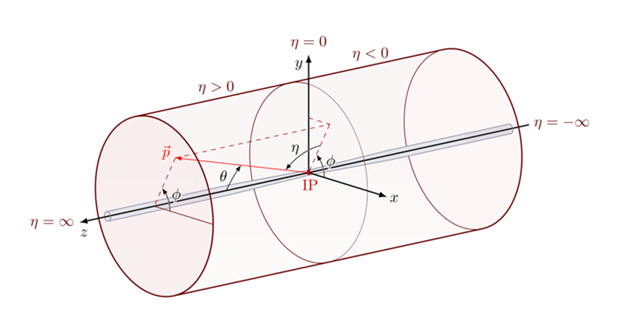
\includegraphics[width=12.5cm,height=6cm]{templates/CMS_coordinates.png}
    \caption{In the LHC, the beam direction is assumed to be in the $z$ axis, and the $x-y$ plane is perpendicular to the beam. $\theta$ is the angle between the particle momentum diirection and the $z$ direction. A particle with energy $E$ and momentum along the beam direction $p_z$ has rapidity $y \equiv \frac{1}{2} \ln \frac{E+p_{x}}{E-p_{x}}$ and pseudorapidity $\eta \equiv-\ln \tan \theta / 2$. Massless particles have $y=\eta$, and differences in rapidity are invariant under longitudinal (along the beam direction) boosts.}
    \label{CMS_coordinates}
\end{figure}
The most efficient and widely-used clustering algorithm is the anti-kt algorithm, usually implemented in the FastJet package.


After jets have been reconstructed, studying them can offer treasure trove of information about fundamental physics. One of the best best studied things in the LHC related to jets is the inclusive jet spectrum, which is related to the momentum transfer $2 \rightarrow 2$ scttering of partons inside the proton. In this process, the energy of a the jet is closely related to that of the hard scattering of partons inside the protons, therefore the inclusive jet spectrum quantifies the distributions of partons inside the proton.




Measurements of the inclusive jet and dijet cross sections are classical particle physics measurements and are benchmarks of the standard model at particle colliders. Such measurements have been measuren in $e^+ e^-, ep, pp,$ and $p \bar{p}$ colliders. They have been used to test the predictions of perturbative QCD, have given precise measurements of the strong coupling constant $\alpha_S$, have been used to obtain information about the structure of the photon and neutron by constraining parton distribution functions (PDFs) of theproton (as well as differentiate between PDF sets), and  have been used to look for possible deviations from the standard model.  








\section{What is a cross section and what are PDFs?}
The total scattering cross section is computed by convoluting the parton distibution function for each incoming parton from each proton with the corresponding partonic level cross section.

Hence, in the language of QCD, the short-distance (high energy) part of the process can be computed from perturbation theory, and long-distance (low energy) part of the process is driven by the non-perturbative nature of QCD at low-energy scales. Collinear factorization theorem allows us to separate the perturbative (calculable) hard part of the process from the non-pertubative one, which can be described in terms of parton distribution (or fragmentation) functions. The total cross section of inelastic proton-proton scattering to produce a final state $n$ can be calculated with the formula
\begin{equation}
    \sigma = \sum_{a, b} \underbrace{\int_{0}^{1} d x_{a} d x_{b} f_{a/A}\left(x_{a}, \mu_{F}\right) f_{b/B}\left(x_{b}, \mu_{F}\right)}_{\text{long-distance, non-perturbative PDF part}} \times \underbrace{\int d \Phi_{n}  \frac{1}{2 \hat{s}}\left|\mathcal{M}_{a b \rightarrow n}\right|^{2}\left(\Phi_{n} ; \mu_{F}, \mu_{R}\right)}_{\text{short-distance "hard" perturbative part}}
    \label{QCD_master}
\end{equation}
Where $f_{a/A}(x, \mu)$ denotes the parton distribution functions, which depend on the momentum fractin $x$ of a parton $a$ with respect to its parent hadron $A$, and on an arbitrary energy scale called the factorization scale $\mu_F$. $d \Phi_{n}$ is the differential phase space element over $n$ final-state particles,
\begin{equation}
    d \Phi_{n}=\prod_{i=1}^{n} \frac{d^{3} p_{i}}{(2 \pi)^{3} 2 E_{i}}(2 \pi)^{4} \delta^{(4)}\left(p_{a}+p_{b}-\sum_{i=1}^{n} p_{i}\right)
\end{equation}
Where $p_a$ and $p_b$ are the initial state momenta. 
The convolution of the squared matrix element $\left|\mathcal{M}_{a b \rightarrow n}\right|^{2}$ 
, averaged over initial-state spin and colour degrees of freedom, with the
Lorentz-invariant phase space Φn and multiplied by the flux factor $ 1/(2ˆs) = 1/(2xaxbs)$
results in the calculation of the parton-level cross section $\hat{\sigma}_{ab→n}$. 

Hence we can intuitively say that the differential cross section in transverse momenta of the observed jet can be factorized in the following form \footnote{sometimes this is called the "master formula"}
\begin{equation}
\frac{d \sigma_{jet}}{d \mathcal{O}} \sim\\
\sum_{a, b} \int d x_{a} f_{a / A}\left(x_{A}, \mu\right) \int d x_{b} f_{b / B}\left(x_{B}, \mu\right) \frac{d \sigma_{partons}}{\mathcal{O}}
\label{master}
\end{equation}
Where $\sigma_{partons}=\int d \Phi_{n}  \frac{1}{2 \hat{s}}\left|\mathcal{M}_{a b \rightarrow n}\right|^{2}\left(\Phi_{n} ; \mu_{F}, \mu_{R}\right)$ can be seen from \ref{QCD_master}, and $ \mathcal{O}$ is any jet observable for example the jet $p_T$ or the rapidity $|y|$. The equation \ref{master} illustrates the principle of \emph{factorization}  i.e. that short distance and long distance processes are separable such that they can be convoluted in this manner, so that the "hard part" $\sigma_{partons}$ and "normalizations" from the PDFs are on diffrent scales.   Factorization also posits that the PDFs are universal, i.e. process-independent. 


The parton level cross sections $d \sigma_{partons}$ has an expansion in powers of $\alpha_S$
\begin{equation}
    \frac{d \sigma_{partons}}{d P_{T}} \sim \sum_{N}\left(\frac{\alpha_{s}(\mu)}{\pi}\right)^{N} H_{N}\left(x_{A}, x_{B}, P_{T} ; a, b ; \mu\right)
    \label{patron_x}
\end{equation}
Where the coefficients $H_N$ are calculable in perturbative QCD. Equation \ref{parton_x} demonstrates the principle of \emph{Asymptotic Freedom}, i.e. hard scattering is weak at short distances, and hence perturbatively calculable. At next-to-leading-order and beyond, however, the calculation will involve divergences that must be removed, and the dependence on the scale $\mu$ will appear in their place. 

% Inclusive jet cross section measurements are typically defined by the anti-$k_T$ algorithm implemented in the FASTJET package. Such an algorithm is infrared-safe and boost-invariant along the z-axis. The algorithm has proven to be the most effective in keeping the background induced from pileup (i.e. from other interactions) under contril by keeping the jets circular in the $(y, \phi)$ plane with a radius radious roughly equal to the jet size parameter $R$.















\section{Short-term and long-term plan for my thesis}
As Run 3 will start later this year, the timing of my dissertation seems apt to analyze Run 1 and
2 data, as well as be one of the first to analyze Run 3 data. Although I have worked and still
work on many different projects in ML, PDFs, HGCAL, database, prefiring, my dissertation
will in a big picture view be composed of two parts: a short-term plan, which I define as my plan up to the next year, and a long-term plan, which is defined as my plan until I graduate, estimated to be 2 or 3 years. 

For my short term plan, I am going to be a part of a team at DESY that will use the full Run 2 dataset to measure the inclusive jet cross section. I plan to go to DESY this summer to work on this project, and our team plans to publish a paper on this measuremtn next year of which I will be one of the main co-authors.

For my long term plan, which will take the bulk of the writing that is to follow, I plan to do my own inclusive jet cross section measurement using the preliminary Run 3 data, but I will be using a novel observable for which there is only a single observable per event. This is done so that we can avoid cross problematic correlations between the different channels/bins. Having measured this cross section over the full $p_T$ range, we will use that to do a EFT fit. The novelty in our EFT fit is that this time we will do a true global fit, without making any assumptions about the EFT coeffiecients. This means that we will fit all the EFT (Wilson) coefficients simultaneously resulting in a full-scale modelling of the probability distributions of the Wilson coefficients. This would give the best chance of saying something about dimension-6 operators that might set bounds on new physics, as well as searching for contact interactions. 
%% \chapter{ My Previous Projects, and How They are Relevant and important}














\section{My previous projects}
This measurement requires many areas of expertise and skill, as it is one of the most difficult and ambitious measurements in modern particle physics. In preparation for this measurement, I have been building my skill sets and expertise in relevant particle physics research areas, here are a few research projects that I've worked on and how they are relevant in my preparation for this measurement.

\section{L1 Prefiring}
 As a member of the JETMET POG, I have worked on the L1 Prefiring problem for data collected in 2017 and 2018, and has made contributions and discoveries that has affected the entire CMS experiment. A brief summary of this issue is the following: from the end of 2016, certain jets and photons in the forward rejoin ($2<|\eta| <3$) were wrongly associated by the L1 trigger to be belonging to the previous bunch crossing, resulting in a loss of these events. This effect cannot be accounted for in MC, therefore a correction to MC must be applied to compensate for this loss of efficiency. A centrally produced map for the UL 2017 dataset was produced by me to account for this inefficiency. The probability map is in the $(p_T, \eta)$ plane of the jets or photons, and the probability of prefiring can be applied to MC jets/photons as weights to account for this inefficiency. Figure \ref{UL_2017} shows an example of the maps that I produced \footnote{These maps can be used for MC correction on CERN website [] }, but the interested reader should read my contributions to the JETMET POG presenting these results \cite{UL2017}. Working on this issue has given me the necessary tools and expertise and experience on how triggering is done in CMS, analyzing the behaviors of the various detectors in detail, as well as contributing to the experiment in a significant way.

\begin{figure}[h]%
    \centering
    \subfloat[\centering]{{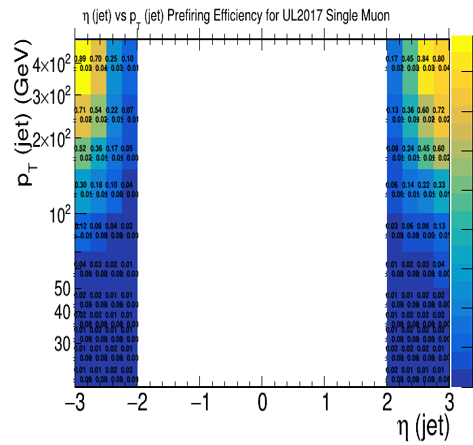
\includegraphics[width=7.05cm,height=6cm]{templates/images/UL17Pref_jetmap.png} }}%
    \qquad
    \subfloat[\centering]{{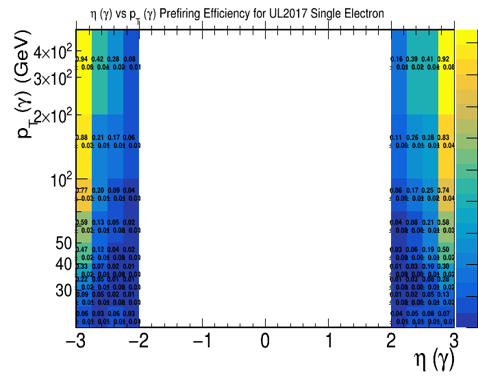
\includegraphics[width=7.05cm,height=6cm]{templates/images/UL17Pref_photonmap.png} }}%
    \caption{UL 2017 Prefiring Maps produced by Myself. The interested reader should also read my JETMET Contribution on this at \cite{UL2017}}%
    \label{UL_2017}%
\end{figure}




Recently, I performed this study again but this time for UL 2018 dataset. Myself and everyone else involved in these studies expected that we would see very small probabilities of prefiring for the UL 2018 data, since this problem was assumed to have been fixed. See for example \cite{Nick_Thomas} which describes how it was fixed. Indeed, my study concluded that this problem was fixed in the L1 trigger as the probabilities of prefired jets and photons were very low, as shown in figure. 
% UL 2018 2D MAPS
\begin{figure}[h]%
    \centering
    \subfloat[\centering]{{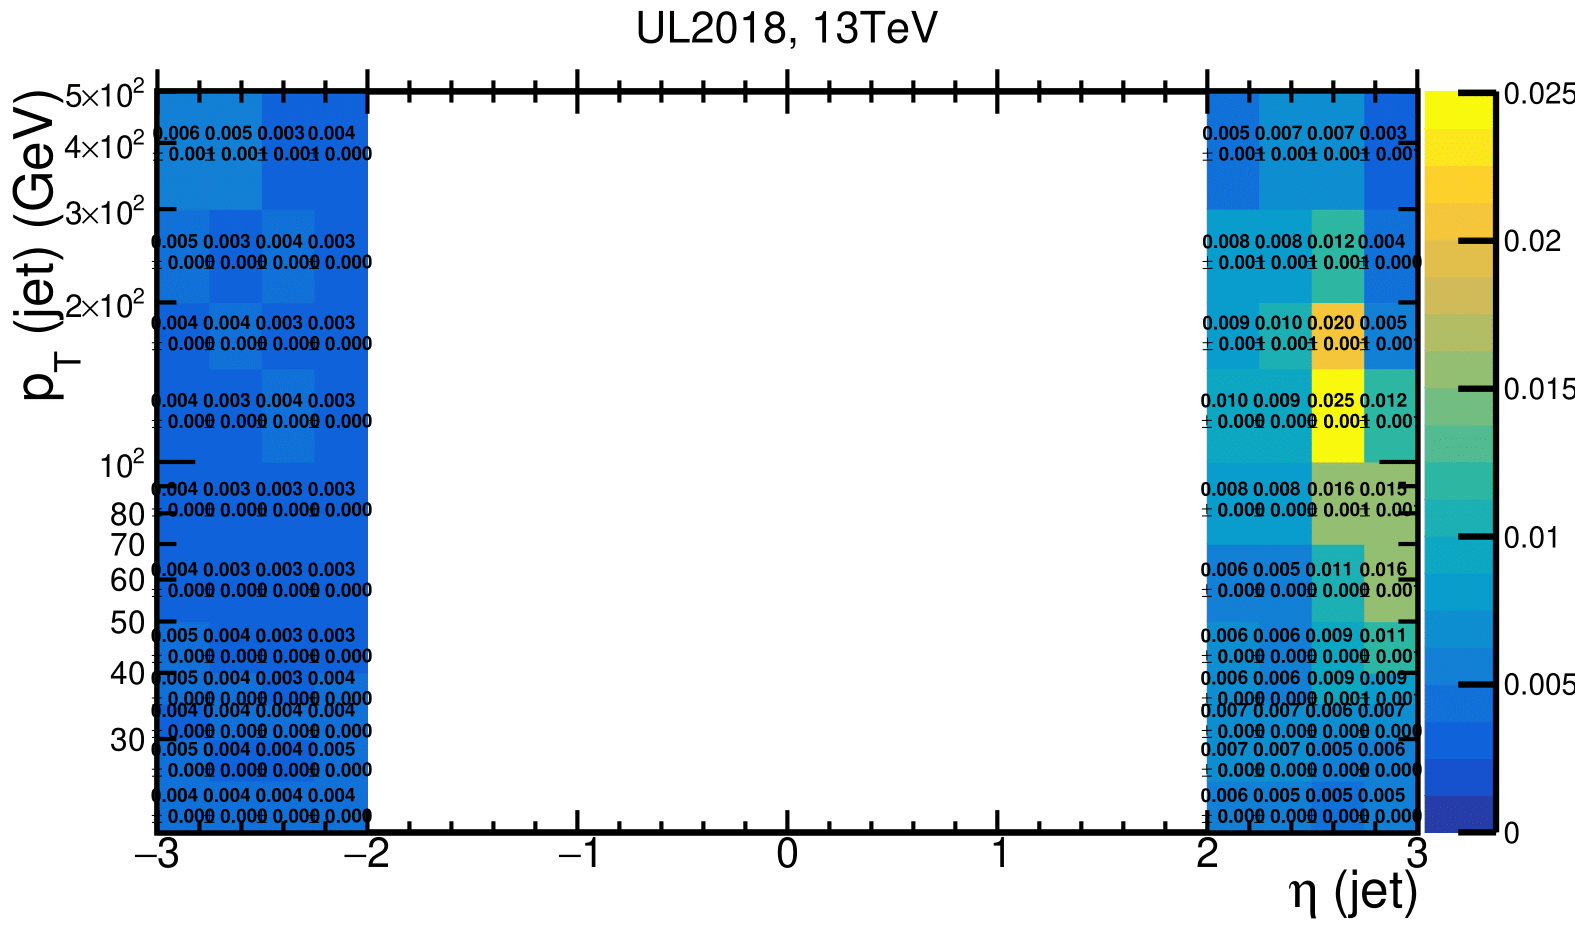
\includegraphics[width=4.5cm,height=5cm]{templates/images/JETptvseta_2D_UL2018-1.png} }}%
    \qquad
    \subfloat[\centering]{{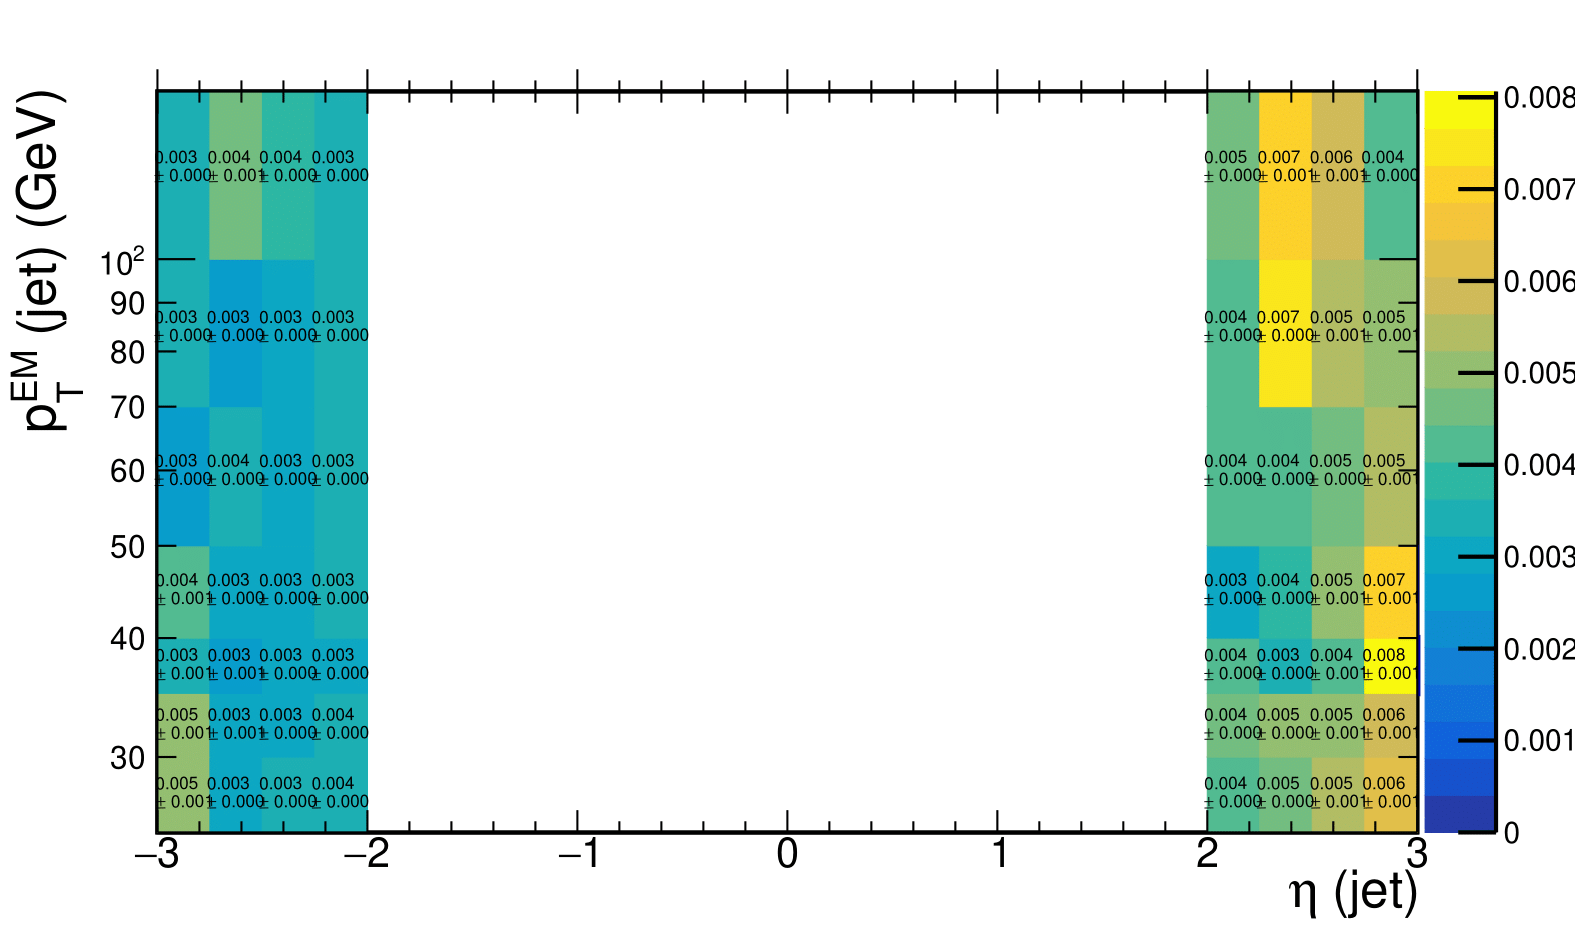
\includegraphics[width=4.5cm,height=5cm]{templates/images/JETEMptvseta_2D_UL2018-1.png} }}%
    \subfloat[\centering]{{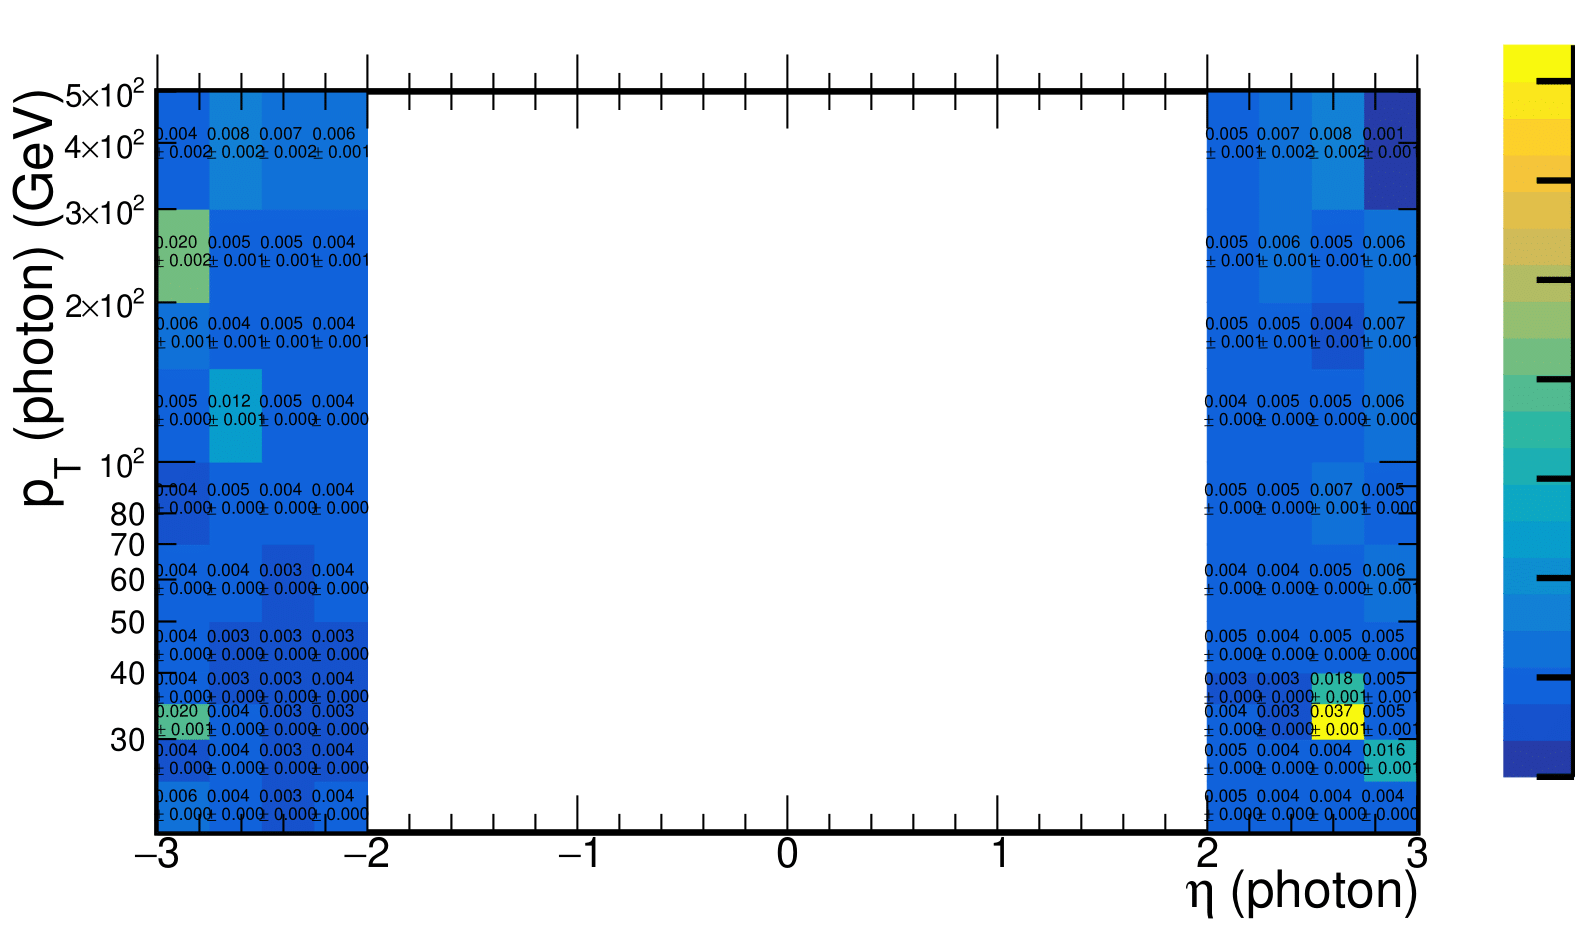
\includegraphics[width=4.5cm,height=5cm]{templates/images/PHOTONptvseta_2D_UL2018-1.png} }}%
    \caption{UL 2018 Prefiring Maps produced by Myself. The interested reader should also read my L1 DPG Contribution on this at \cite{UL2018}}%
    \label{UL_2018}%
\end{figure}

My studies on prefiring during 2018 showed two things that were unexpected. First, although the probabilities of prefiring were low overall, there was clear assymetry in prefiring probabilities for the $\eta>0$ region compared to the $\eta<0$ region (previously it was completely symmetric in $\eta$ previously, as sen in figure \ref{UL_2017}). This can be seen in figure \ref{UL_2018_RunA}. The other surprising thing was that the residual evident prefiring was coming from Run A, with a clear $\eta/ \phi$ structure, as seen in figure \ref{UL_2018_RunA}. Furthermore, I found that these effects were coming from two runs numbers in Run A where the L1 trigger misbehaved. My analysis was later fully confirmed by L1 DPG (see \cite{L1DPG}) by a different method, and as a result we removed these bad runs from the Golden JSON for 2018, affecting the entire CMS experiment.

%UL 2018 Run A
\begin{figure}[h]%
    \centering
    \subfloat[\centering Ratio efficiencies jets]{{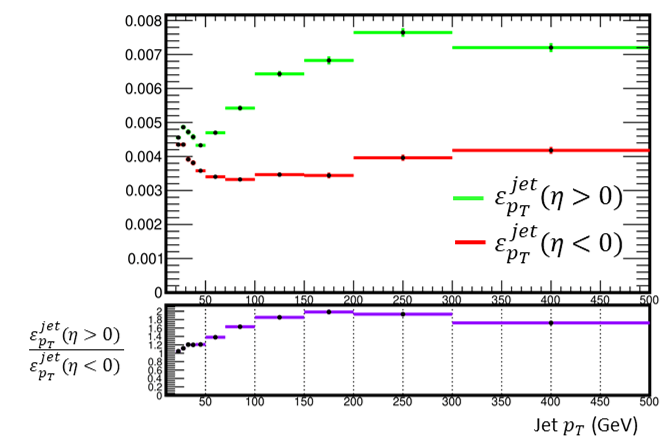
\includegraphics[width=5cm,height=5cm]{templates/images/Ratio_of_efficiencies_JETPT.png} }}%
    \qquad
    \subfloat[\centering Ratio of efficiences photon]{{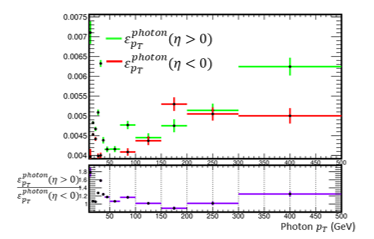
\includegraphics[width=5cm,height=5cm]{templates/images/Ratio_of_efficiencies_PHOTONPT.png} }}%
    \subfloat[\centering 1D hists]{{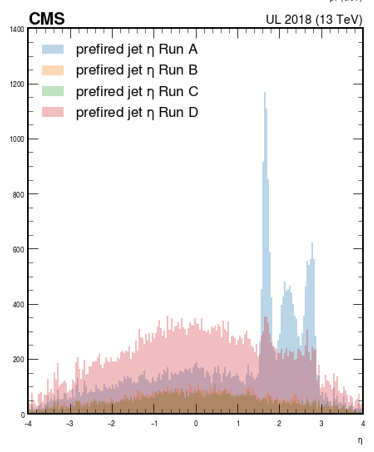
\includegraphics[width=5cm,height=5cm]{templates/images/1DHISTS_UL2018.png} }}%
    \subfloat[\centering Run A eta vs phi]{{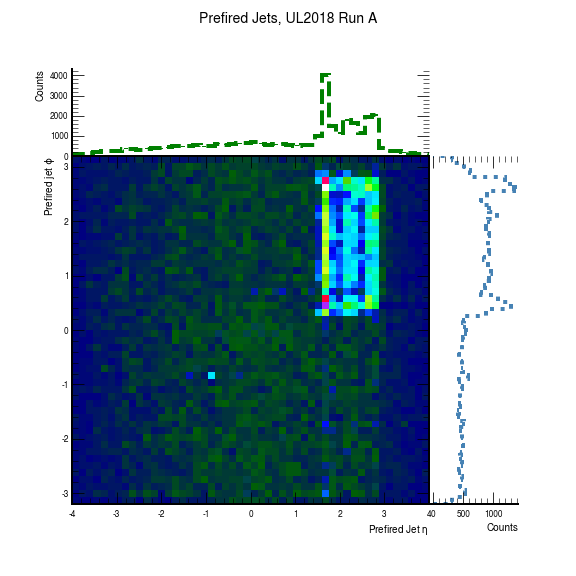
\includegraphics[width=5cm,height=5cm]{templates/images/Jet_phi_vs_eta_runA_PREFIRED.png} }}%
    \caption{UL 2018 Prefiring Maps produced by Myself. The interested reader should also read my L1 DPG Contribution on this at \cite{UL2018}}%
    \label{UL_2018_RunA}%
\end{figure}




As discussed in Chapter 1 (sec on the uncertainties included), there are many uncertainties and inefficiencies that enter the jet cross section measurement, and this is one of the inefficiencies that enter the calculation which has to be accounted for. Since I will be using Run 2 Data, correcting for this effect for my short-term plan will be crucial. 


\section{PDFs and xFitter}

As shown in Ch.1 sec on PDFs, PDF are paramount in jet cross section measurement and in any cross section measurement. Since there are many groups that routinely publish different PDF sets, a big problem in HEP is the proper characterization of these different PDFs and the quantification of their uncertainties and the uncertainties of the parameters that are included in different PDF sets, which was the aim of my studies in PDFs, where I used the PDF fitting software xFitter.

As discussed below, the reported PDF uncertainties and confidence intervals make some assumptions regarding the parameterization of the PDFs, which may not be statistically justified. A popular method for estimating the PDF errors is by constructing confidence intervals on the parameters using $-2 \log L$: suppose that the likelihood for $\theta$ is multivariate normal, the likelihood function of a single observation is of the form 
\begin{equation}
\begin{aligned}
    L(\boldsymbol{\theta} ; x)&=\frac{1}{\sqrt{(2 \pi)^{D}|\boldsymbol{\Sigma}|}} \exp \left\{-\frac{1}{2}[x-g(\boldsymbol{\theta})]^{T} \boldsymbol{\Sigma}^{-1}[\boldsymbol{x}-\mathrm{g}(\boldsymbol{\theta})]\right\} \\
    &= \frac{1}{\sqrt{(2 \pi)^{D}|\boldsymbol{\Sigma}|}} \exp \left\{-\frac{1}{2}\chi^2\right\}
\end{aligned}
\end{equation}
Taking the log and dropping the constant in the beginning (since the constant is independent of $\theta$), we have
\begin{equation}
\begin{aligned}
    \log L(\boldsymbol{\theta} ; \boldsymbol{x})&=-\frac{1}{2}[\boldsymbol{x}-\mathrm{g}(\boldsymbol{\theta})]^{\mathrm{T}} \boldsymbol{\Sigma}^{-1}[\boldsymbol{x}-\mathrm{g}(\boldsymbol{\theta})] \\
    &= - \frac{1}{2} \chi^2
\end{aligned}
\end{equation}

Thus, $-2 \log L$ is precisely the $\chi^2$ expression in the leaset squares method.
A popular method for estimating the errors in the maximum likelihood method is to look for parameters $\mathbf{\theta_{\pm}}$ for which
\begin{equation}
    -2 \Delta \log L \equiv-2\left[\log L\left(\boldsymbol{\theta}_{\pm} ; \boldsymbol{x}\right)-\log L(\hat{\boldsymbol{\theta}} ; x)\right]=1
\end{equation}
This method yields 68 \% confidence intervals on the individual parameters. These shifts in the parameters $\boldsymbol{\theta_{\pm}}$ can be attained with the maximum likelihood methodology. In other words, finding the points where $\Delta \chi^2=1$ corresponds to the method of finding the 68 \% confidence interval $( \hat{\theta} - \theta_+, \hat{\theta} + \theta_+ )$.

This method is widely used by all PDFs, but it is critical to remember that this assumes the normal sampling of $x$. If the sampling is not normal, then the probability content will be different, and must be determined for the correct sampling distribution. Since this method is used by xFitter and most other PDF fitting tools, we aim to study this assumption, whether it is true that the parameters that we aim to study are normally distributed. 

Our study aims at studying to what extent the PDF parameter marginalized densities (distributions) are normal (which is what PDF groups imply as discussed above), and whether we can retreive the actual parameter likelihoods, which might not be Gaussian, by a reweighting technique. We reweight the parameter points $\theta_i$ by the weight $w_i = \frac{L(\theta_i)}{\pi (\theta_i)}$ where $L(\theta_i)$ is the true likelihood for parameter $\theta$ at point $i$ and $\pi(\theta_i)$ is a prior or approximate likelihood of our choice, which assume $\Delta \chi^2 =1$. For example we could take it to be a multivariate Gaussian $\pi(\theta_i) = \mathcal{N} (\mu = \hat{\theta_i}, \Sigma = \hat{\Sigma})$, where $\hat{\theta_i}$ and $\hat{\Sigma}$ are the best-fit PDF values and their covariance matrix that are returned by xFitter, respectively. Our method shows promise for working in the limit of increasing datasets included in the PDF fit, due to the descrepancies between the different experiments which would affect the noramlity of the parameter distributions. For more details, please visit my Github repository, where all the code is available[], and to my invited talk at the 2022 xFitter Workshop \cite{xFitterWorkshop}.











%%%%%%%%%%%%%%%%%%%%%%%%%%%%%%%%%%%%%%%%%%%%%%%%%%%%%%%%%%%%%%%%%%%%%%%%%%%%%%%%%
\section{Quark/Gluon Jet Discrimination with ML}
The identification the origin of jets; whether they are quark or gluon jets, is an extremely important experimental test in uncovering the fundamental physics that occurs in a given event. One of the areas where quark-gluon jet identification is important is in understanding the properties of the Higgs. For example, if one wants to measure the Higgs boson coupling to gauge bosons, one would need to look at the weak-boson-fusion process $qq \rightarrow H qq$ (which makes quark jets) and not the more frequent gluon-fusion process $gg \rightarrow Hgg$ (which generates a gluon jet). In this project I used CMS Open Data to build machine learning classification models to classify between quark or gluon initiated jets. Using Baye's Theorem, $p(y \mid x)=\frac{p(x \mid y) p(y)}{p(x)}$ we therefore have the probability of observing a gluon jet given data $x$ as $p(\text{ gluon } |x) =\frac{p(x \mid \text { gluon }) p(\text { gluon })}{p(x \mid \text { gluon }) p(\text { gluon })+p(x \mid q u a r k) p(\text { quark })} $ which is the outcome of our ML classifier. An ensemble of all the state-of-the art classifiers that are available in common ML packages was studied in application to this problem, and the ML hyperparameters were all tuned to their optimal values using random grid search. The best performing classifier, as indicated by the ROC curves in figure \ref{ROC_QG}. Perhaps more interestingly, I found that the jet observable that resulted in the greatest discrimination power between quark and gluon jets was the jetQCI variable, which was constructed on the basis that gluon jets are wider than quark jets, as seen in figure \ref{QGI}. see \cite{QGI} for more details.

\begin{figure}[h]%
    \centering
    \subfloat[\centering ROC Curves for classifiers whose hyperparameters were tuned with grid search]{{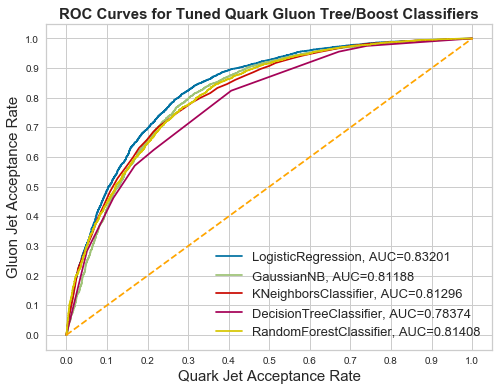
\includegraphics[width=7cm,height=5cm]{templates/ROC_TUNED.png} }}%
    \qquad
    \subfloat[\centering The jet observables that yield the greatest discrimination power between quark and gluon jets. The winner is the jetQGI variable, which is denoted as $\sigma$ in \cite{QGI}]{{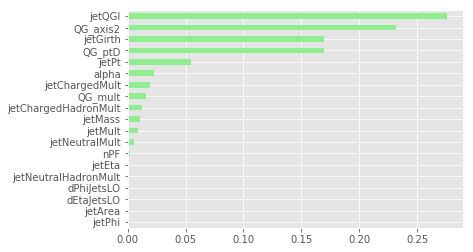
\includegraphics[width=7cm,height=5cm]{templates/images/feature_importance.png} }}%
    \caption{UL 2017 Prefiring Maps produced by Myself. The interested reader should also read my JETMET Contribution on this at \cite{UL2017}}%
    \label{QGI}%
\end{figure}
This study was later extended to consider a more realistic model for quarks and gluons. Recall that the objective of any classifier is to approximate the function 
\begin{equation}
    \begin{aligned}
f^{*} &=P(t=1 \mid x) \\
&=\frac{p(x \mid s) \pi(s)}{p(x \mid s) \pi(s)+p(x \mid b) \pi(b)}
\end{aligned}
\end{equation}

In other words, the function $f^∗$ (or classifier) approximates the discriminant
\begin{equation}
    D(x)=\frac{s(x)}{s(x)+b(x)}
\end{equation}

However, this discriminant assumes ideal and \emph{pure} probability densities $g(x)$ and $q(x)$. The actual densities of the samples have quark densities that include mixtures of the other quark flavor, and since we are only considering binary classification of quark and gluon jets, the actual densities are
\begin{equation}
\begin{aligned}
&G(x)=\left(1-\epsilon_{q}\right) g(x)+\epsilon_{q} q(x) \\
&Q(x)=\left(1-\epsilon_{g}\right) q(x)+\epsilon_{g} g(x)
\end{aligned}
\end{equation}
Where the fractions $\epsilon_g$ and $\epsilon_q$ are mixture fractions corresponding to the two jet flavors. Hence we can define the actual, or \emph{contaminated discriminant} $D'(x)$, which is what we are actually approximating by the classifiers, which includes the mixture fractions
\begin{equation}
    D^{\prime}(x)=\frac{G(x)}{G(x)+Q(x)}
\end{equation}
Which, after subsitituting $G$ and $Q(x)$ and simplifying
\begin{equation}
    D^{\prime}(x)=\frac{\epsilon_{q} q(x)_{g}(x)\left(1-\epsilon_{q}\right)}{\epsilon_{g} g(x)-\epsilon_{g}+\epsilon_{q} q(x)+g(x)\left(1-\epsilon_{q}\right)+1}
\end{equation}
Now, what is interesting is that $D'(x)$ can be represented in terms of $D(x)$
\begin{equation}
    D^{\prime}=D \frac{(g+q)(e q q+g(1-e q))}{g(e g g-e g+e q q+g(1-e q)+1)}
\end{equation}
This means that the realistic contaminated discriminant is a function of $D$ only since $\epsilon_q$ and $\epsilon_g$ are constants. Furthermore, the fact that $D'$ is one-to-one with $D$ means that their discrimination power is the same.  This means that the optimal discriminant $D$ can be computed from
$D'$, where the contamination fractions are given in $D'$
, and by studying the relationship between $D$ and $D'$ over the range of $\epsilon_q$ and $\epsilon_g$ one could identify where
the relationship between them is monotonic.

This project was one of my first applications of machine learning to a particle physics problem and it yielded some interesting results, and a possibility of arriving at an optimal quark-gluon classifier by the contaminated classifier technique described above. It also taught me the power of machine learning in jet studies and how one has freedom to construct jet observables, which becomes all the more powerful if it is informed by intuition and machine learning. Constructing similar observable will be very important for my thesis plan.




%%%%%%%%%%%%%%%%%%%%%%%%%%%%%%%%%%%%%%%%%%%%%%%%%%%%%%%%%%%%








\section{Observable with high $p_T$ jets and the Response Matrix}
\label{jet_order_response}

My goal first in this project was to explore and quantify to what extent the $p_T$ of highest-$p_T$ jet in an event can be used as an observable. My second goal was to study how we can construct the "response matrix" which is a mapping from "true" or theoretical (or generated - gen for short) values to the measured (or reconstructed - rec for short) values, in the context of the jet $p_T$. In CMS analyses, this mapping is done via
\begin{equation}
    \mathbb{P}\left(p_{T}^{\text {rec }} \mid p_{T}^{g e n}\right)=   \mathbb{P}\left(p_{T}^{\text {gen }} \mid \mathrm{SF} \right)
    \times\left(1+\mathrm{SF} \times \Delta_{\mathrm{MC}} R_{G}\right)
\end{equation}
Where $\Delta_{\mathrm{MC}}    =\frac{p_{T}^{\mathrm{rec}}-p_{T}^{\mathrm{gen}}}{p_{T}^{\mathrm{gen}}}$ is the "resolution", $R_G$ is a random number sampled from a standard normal distribution \footnote{meaning $\mu=0, \sigma=1$} and \mathrm{SF} are smearing factors which are extracted from the measurement of the resolution of the data, and are provided centrally at CMS by JetMET. We argue that this mapping makes unproven assumptions (such as the normality of the smearing) and it requires exact knowledge of the smearing factors, which are nuissance parameters, making it very inconvenient.




In our study, we aim to "fold" the gen jet ($p_T$) spectrum by the respense function  $\mathbb{R}\left(p_{T}^{r e c} \mid p_{T}^{\text {gen }}\right)$ by calculating the integral 
\begin{equation}
    \mathbb{P}\left(p_{T}^{\text {rec }} \mid p_{T}^{g e n}\right)=\int \mathbb{R}\left(p_{T}^{r e c} \mid p_{T}^{g e n}\right) f\left(p_{T}\right) d p_{T}
\end{equation}
Where $f(p_T)$ is the true spectrum of the leading jet. The Data is consistent of pythia 8 (CUEITP8M1) MC samples with $2 \rightarrow 2$ parton-parton interactions included
in the matrix element (ME): these will be referred to as ”gen” or generator (truth) samples. \footnote{Multiparton interaction, initial state
radiation, FSR and hadronization were also simulated in the MC samples}
In order to study the detector-related effects, the CMS detector
response is also simulated using the GEANT4 package. These will be referred to as the ”rec” samples. The distributions for the jet kinematic variables $\left(p_{T}, \eta, \phi\right)$ were constructed for $\approx$ 9 Million events, each having a varying number of jets per event. Before we are able to to further analyze these samples and assess the detector response, we must have a one-to-one mapping of each gen jet to its corresponding rec jet. This is done via matching in $(\eta, \phi)$ space, where the distance between a gen (1) jet and a rec (2) jet was chosen nto be within a cone of radius $\Delta R_{12}=\sqrt{\Delta y_{12}^{2}+\Delta \phi_{12}^{2}} < 0.25$.

In order to study the kinematic variables of the reco and gen jets, we can
use the $p_T$ ordering of the jets as a means to quantify whether the $p_T$ of the highest jet can be used as an observable. One way to tell whether it can be used as an observable is to calculated the probability of flipping of the order of the gen jets compared to rec jets, $\mathbb{P}_{f l i p}(g e n, r e c)$: what is the probability that the order of the $p_T$ of the rec jets is flipped when ordered according to the $p_T$ order of the gen jets?

Hence, if we show that there is a nonzero flipping probability for the first jet, i.e. there is a probability that the leading gen jet corresponds to a non-leading reco jet, the response
function has to be modified in order to be compared to the provided
theoretical distribution by multiplying the integral by a flipping probability
\begin{equation}
    \mathbb{P}\left(p_{T}^{r e c} \mid p_{T}^{g e n}\right)=\int \mathbb{R}\left(p_{T}^{r e c} \mid p_{T}^{\text {gen }}\right) f\left(p_{T}\right) \mathbb{P}_{f l i p}\left(p_{T}^{r e c}, p_{T}^{g e n}\right) d p_{T}
\end{equation}

For our task, we want to find the conditional distribution $\mathbb{P}\left(p_{T}^{r e c} \mid p_{T}^{g e n}\right)$. This can be done via a Machine Learning and a "likelihood ratio trick" (see for example [arXiv:1805.12244v4] which also uses this in a HEP application). Given a classification model, which tries to find the mapping $p_T^{rec} = f(p_T^{gen})$, which can be estimated as $\hat{f}$

\begin{equation}
f(p_T^{rec}) \approx \hat{f}(p_T^{gen})=\arg _{\hat{f}} \min \int L(p_T^{rec}, \hat{f}) \ p(p_T^{rec} | p_T^{gen}) d y
\end{equation}
Where $ L(p_T^{rec}, \hat{f})$ is a (binary classification) loss function.

Hence our task is to approximate the optimal classifier, which, given training data $x$ learns

\begin{equation}
d(x)=\frac{\mathbb{P}\left(x | p_T^{rec}\right)}{\mathbb{P}\left(x | p_T^{gen}\right)+\mathbb{P}\left(x | p_T^{rec}\right)}=\frac{f(x)}{1+f(x)}
\end{equation}


Where $f$ is the classifier decision function, Which is 1-to-1 with the likelihood ratio,
\begin{equation}
\hat{r} (x| p_T^{gen}, p_T^{rec})=\frac{\mathbb{P}\left(x | p_T^{rec}\right)}{\mathbb{P}\left(x | p_T^{gen}\right)}
\end{equation}
Which can be written as 

\begin{equation}
\hat{r} (x| p_T^{gen}, p_T^{rec})=\frac{\mathbb{P}\left(x | p_T^{rec}\right) \ \mathbb{P}(p_T^{rec})}{\mathbb{P}\left(x | p_T^{gen}\right) \ \ \mathbb{P}(p_T^{rec})} =\frac{d(x)}{1-d(x)}
\end{equation}
Our posterior density could finally be calculated as
\begin{equation}
    \mathbb{P}\left(p_{T}^{r e c} \mid p_{T}^{g e n}\right)=\frac{d}{1-d} \times f\left(p_{T}^{r e c}\right)
    \label{ratio_trick_posterior}
\end{equation}

In building our probabilistic machine learning model, we have the target class corresponding to the true $p_T^{gen}$ and the normalized distribution of the rec jets $Z= \frac{p_T^{rec}}{p_T^{gen}}$
\begin{equation}
    \left\{p_{T}^{\text {gen }}, Z=\frac{p_{T}^{r e c}}{p_{T}^{\text {gen }}}\right\}, \text { Target }=1
\end{equation}
And the other class corresponding to a distribution that is randomly sampled from $p_T^{gen}$ and a random sampling of the $Z$ distribution, $f(Z)$:
\begin{equation}
    \left\{f\left(p_{T}^{g e n}\right), f(Z)=f\left(\frac{p_{T}^{r e c}}{p_{T}^{g e n}}\right)\right\}, \text { Target }=0
\end{equation}
We pick $f(Z)$  to be randomly sampled from a Gaussian with mean $\mu=\frac{p_{T}^{r e c}}{p_{T}^{\text {gen }}}$ and standard deviation corresponding to the width of the $Z$ distribution, i.e.
\begin{equation}
f(Z)=\frac{1}{\sigma \sqrt{2 \pi}} e^{-\frac{1}{2}\left(\frac{p_T^{rec}-p_T^{gen}}{\sigma}\right)^{2}}
\end{equation}
Therefore the function $f(Z)$ can be regarded as a rough approximation of the distribution $Z$, and given this, $\frac{d}{1-d}$ fixes the approximation.

The posterior distribution from our model in equation \ref{ratio_trick_posterior} was compared to the simulated data which corresponds to the true CMS detector response. These "data" were simulated with Delphes by passing the truth distribution (which was generated with Pythia) to Delphes to reconstruct the jets given the detector response and smearing, using the CMS card. Results using this method is shown in figure

\begin{figure}[h]%
    \centering
    \subfloat[\centering]{{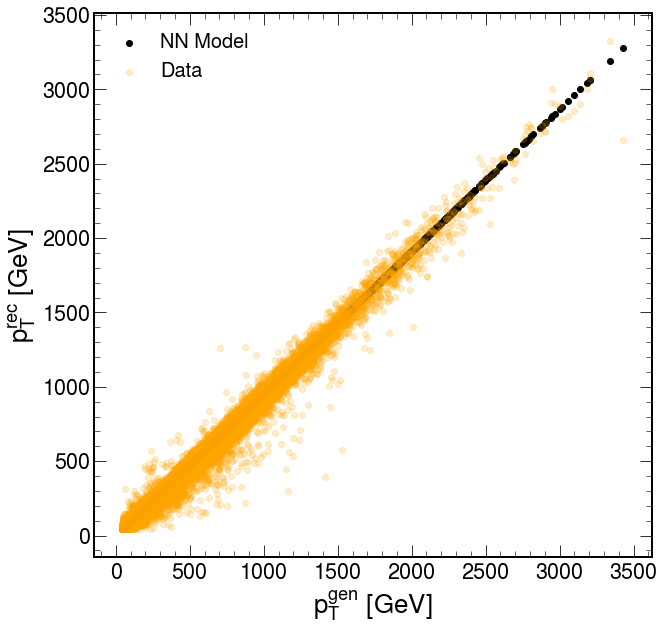
\includegraphics[width=4.5cm,height=5cm]{templates/NN_data_dist.png} }}%
    \qquad
    \subfloat[\centering]{{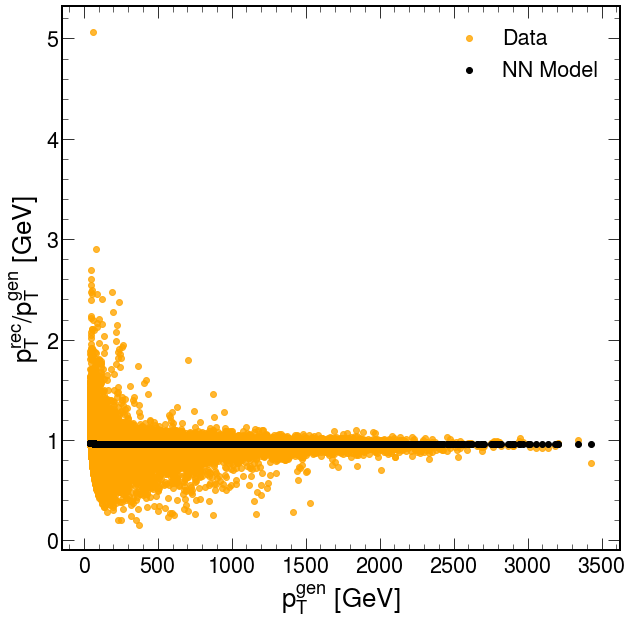
\includegraphics[width=4.5cm,height=5cm]{templates/re_div_gen_model_data.png} }}%
    \subfloat[\centering]{{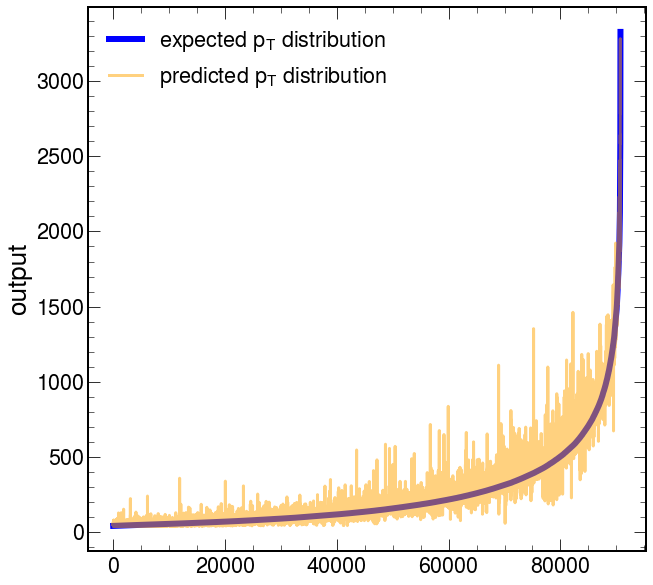
\includegraphics[width=4.5cm,height=5cm]{templates/expected_dist_pt.png} }}%
    \caption{(a): "Response matrix" for matched jets }%
    \label{ratio}%
\end{figure}





















%% \appendix
%% \chapter{Tables}

\begin{table}
\caption{Armadillos}
\label{arm:table}
\begin{center}
\begin{tabular}{||l|l||}\hline
Armadillos & are \\\hline
our	   & friends \\\hline
\end{tabular}
\end{center}
\end{table}

\clearpage
\newpage

%% \chapter{Figures}

\vspace*{-3in}

\begin{figure}
\vspace{2.4in}
\caption{Armadillo slaying lawyer.}
\label{arm:fig1}
\end{figure}
\clearpage
\newpage

\begin{figure}
\vspace{2.4in}
\caption{Armadillo eradicating national debt.}
\label{arm:fig2}
\end{figure}
\clearpage
\newpage

%% %% This defines the bibliography file (main.bib) and the bibliography style.
%% If you want to create a bibliography file by hand, change the contents of
%% this file to a `thebibliography' environment.  For more information 
%% see section 4.3 of the LaTeX manual.
\begin{singlespace}
\bibliography{main}
\bibliographystyle{plain}
\end{singlespace}

%% \end{document}

%% Comment: to include appendices use a single \appendix command followed 
%% by a number of \include{} commands as many files as needed, each of 
%% which should contain a \chapter{} command for the appendix title.
